\documentclass[11pt]{article}
\usepackage{acl2016}
\usepackage{url}
%\usepackage{latexsym}
\usepackage[T1]{fontenc}
\usepackage{times}
\usepackage[utf8]{inputenc}
\usepackage[english]{babel}
\usepackage{natbib}
\usepackage{hyperref}
\usepackage{amsmath,amssymb,amsfonts,amsthm,amstext,amscd}
%\usepackage[usenames, dvipsnames]{color}

%\newcommand{\huang}{\texttt{huang}}
\newcommand{\neelakantan}{\cite{Neelakantan:2014}}
\newcommand{\adagram}{\texttt{AdaGram}}
\newcommand{\mutli}{\texttt{mutli}}
\newcommand{\Ro}{\mathbb{R}^{d_1}}
\newcommand{\Rt}{\mathbb{R}^{d_2}}
\newcommand{\fl}{\texttt{4lang}}

\usepackage{tikz}
\definecolor{hltblue}{RGB}{3,61,92}
\definecolor{hltdarkgreen}{RGB}{26,148,129}
\definecolor{hltlightgreen}{RGB}{155,204,147}
\definecolor{hltyellow}{RGB}{252,238,166}

\usepackage{booktabs}
%\usepackage{multirow,multicol}
\usepackage{cleveref}
%\usepackage{graphicx}
%\usepackage{dblfloatfix}
%\usepackage{array}
%\usepackage{changepage}

\hyphenation{poly-semy}
%\usepackage{dcolumn}
%\newcolumntype{d}[1]{D{.}{.}{#1}}

%\usepackage{todonotes}

\aclfinalcopy % Uncomment this line for the final submission
%\def\aclpaperid{28} %  Enter the acl Paper ID here

%\setlength\titlebox{8cm}
%\setlength\titlebox{50ex}  % Vertical space allocated for \Authors
% You can expand the titlebox if you need extra space
% to show all the authors. Please do not make the titlebox
% smaller than 5cm (the original size); we will check this
% in the camera-ready version and ask you to change it back.

\title{Do multi-sense embeddings learn more senses? \\ An evalutaion in linear
translation}
\author{
  Márton Makrai
  %\\ Institute for Linguistics\\
  %Hungarian Academy of Sciences \\
  %Bencz\'ur u. 33 \\ 1068 Budapest, Hungary \\
  %{\tt makrai.marton@nytud.mta.hu} \\
}
\date{}


\begin{document}
\maketitle

%\hspace{2cm}

%\begin{abstract}
%\end{abstract}

\emph{Word sense induction} (WSI) is the task of discovering senses of words
without supervision \citep{Schutze:1998}. Recent approaches include multi-sense
word embeddings (MSEs), vector space models of word distribution with more
vectors for ambiguous words, each vector corresponding ideally to a different
word sense.

In \cite{Borbely:2016}, we proposed a cross-lingual method for the evaluation
of MSEs based on the principle that words may be ambiguous as far as the
postulated senses translate to different words in some other language.  We
applied the method by \citet{Mikolov:2013x} who train a translation mapping
from the source languages embedding to the target as a least-squares regression
supervised by a seed dictionary of the  few thousand most frequent words. The
translation of a source word vector is the nearest neighbor of its image by the
mapping in the target space. In the multi-sense setting, we translated from
MSEs (the target embedding remaining single-sense).

Now we develop the eveluation further. Part of the eveluation task is to decide
on empirical grounds whether different good translations of a word are synonyms
or translations in different senses.  We analyze sense vectors based on their
distance, which is not directly determined by the distance of the sense vectors
in the source space because of the nearest neighbor search.

The code for these experiments can be found at
\url{https://github.com/makrai/wsi-fest}

\section{%Monosemy:
  Towards a less delicious
  %sense
  inventory}

\begin{figure}[b]
    \centering
    \resizebox{\columnwidth}{!} {
        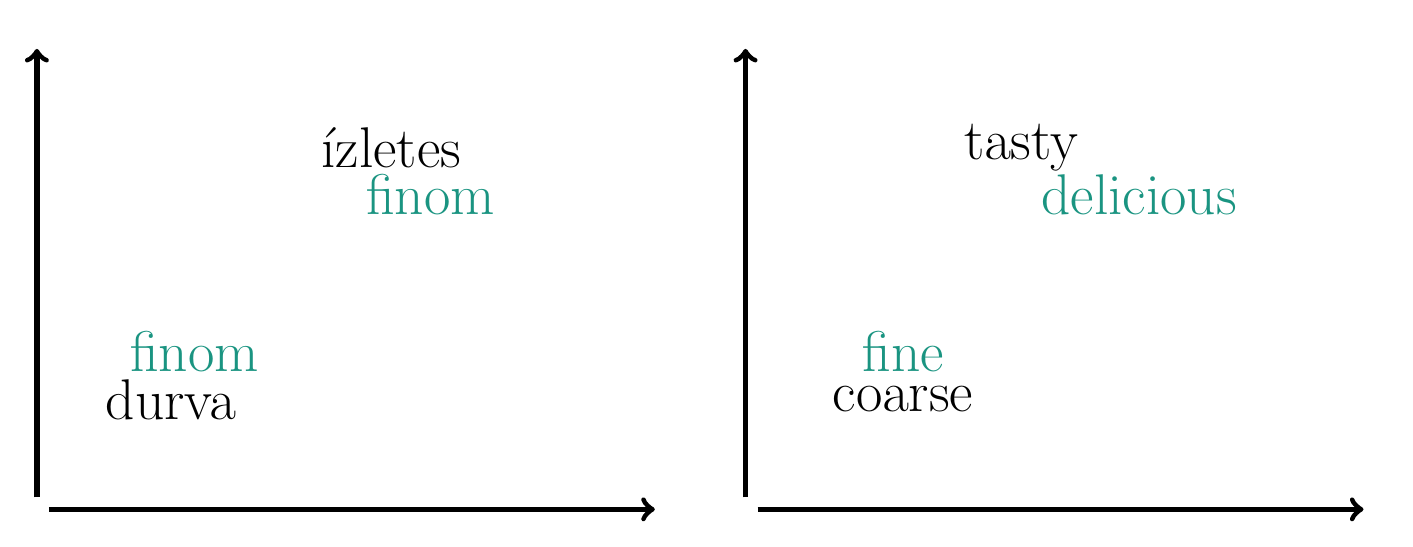
\begin{tikzpicture}[line width=2pt] %[&gt;=stealth']
            \tikzstyle{every node}=[font=\huge]
            %\tikzset{every edge thick}
            \node[text=hltdarkgreen] (hf) at (2, 2) {finom};
            \node (hf) at (1.7, 1.4)  {durva};
            \node[text=hltdarkgreen] (hs) at (5, 4)  {finom};
            \node (hs) at (4.5, 4.6)  {ízletes};
            \node[text=hltdarkgreen] (gf) at (11, 2) {fine};
            \node (gf) at (11, 1.4) {coarse};
            \node[text=hltdarkgreen] (gs) at (14, 4) {delicious};
            \node (gs) at (12.5, 4.6) {tasty};
            \node (ho) at (0, 0) {};
            \node (hx) at (8, 0) {};
            \node (hy) at (0, 6) {};
            \node (go) at (9,0) {};
            \node (gx) at (17,0) {};
            \node (gy) at (9,6) {};

            \draw[->] (ho) edge (hx);
            \draw[->] (ho) edge (hy);
            \draw[->] (go) edge (gx);
            \draw[->] (go) edge (gy);
        \end{tikzpicture}
    }
    \caption{Linear translation of word senses. The Hungarian word
        \emph{finom} is ambiguous between `fine' and `delicious'.}
        \label{fig:AdaGram}
\end{figure}

The differentiation of word senses, as already noted in \cite{Borbely:2016}, is
fraught with difficulties, especially when we wish to distinguish homophony,
using the same written or spoken form to express different concepts, such as
Russian {\it mir} `world' and {\it mir} `peace' from polysemy, where speakers
feel that the two senses are very strongly connected, such as in Hungarian {\it
nap} `day' and {\it nap} `sun'.  To quote \cite{Zgusta:1971} ``Of course it is
a pity that we have to rely on the subjective interpretations of the speakers,
but we have hardly anything else on hand''. %Etymology makes clear that
Different languages make different lump/split decisions in the conceptual
space, so much so that translational relatedness can, to a remarkable extent,
be used to recover the universal clustering \citep{Youn:2016}.
\Cref{sec:bground} offers an overview by Veronika Lipp.

\subsection{Lexicographic Background \\ (Veronika Lipp)}

\label{sec:bground}

Lexical ambiguity is linguistically subdivided into two main categories:
\emph{homonymy and polysemy} \citep{Cruse:2004}. Homonymous words have
semantically unrelated and mutually incompatible meanings, such as
\emph{punch$_1$} , which means `a blow with a fist', and \emph{punch$_2$},
which means `a drink'. Some have described such homonymous word meanings as
essentially distinct words that accidentally have the same phonology (e.g.,
Murphy, 2002). Polysemous words, on the other hand, have semantically related
or overlapping senses (\cite{Cruse:2004,Jackendoff:2002, Pustejovsky:1995}),
such as \emph{mouth} meaning both `organ of body' and `entrance of cave'.

Two criteria have been proposed for the distinction between homonymy and
polysemy. The first criterion has to do with the \emph{etymological} derivation
of words. Words that are historically derived from distinct lexical items are
taken to be homonymous. However, the etymological criterion is not always
decisive. One reason is that there are many words whose historical derivation
is uncertain. Another reason is that it is not always very clear how far back
we should go in tracing the history of words \citep{Lyons:1977}.

The second criterion for the distinction between homonymy and polysemy has to
do with the \emph{relatedness/unrelatedness of meaning}.  The distinction
between homonymy and polysemy seems to correlate with the native speaker’s
feeling that certain meanings are connected and that others are not. Generally,
unrelatedness in meaning points to homonymy, whereas relatedness in meaning
points to polysemy.  However, in a large number of cases, there does not seem
to be an agreement among native speakers as to whether the meanings of the
words are related. So, it seems that there is not a clear dichotomy between
homonymy and polysemy, but rather a continuum from ‘‘pure’’ homonymy to
‘‘pure’’ polysemy \citep{Lyons:1977}.

Most discussions about lexical ambiguity, within theoretical and computational
linguistics, concentrate on polysemy, which can be further divided into two
types (c.f. \cite{Apresjan:1974,Pustejovsky:1995}). The first type of polysemy
is motivated by \emph{metaphor (irregular polysemy)}. In metaphorical polysemy,
a relation of analogy is assumed to hold between the senses of the word. The
basic sense of metaphorical polysemy is literal, whereas its secondary sense is
figurative. For example, the ambiguous word \emph{eye} has the literal basic
sense  `organ of the body' and the figurative secondary sense `hole in a
needle.' The other type of polysemy is motivated by \emph{metonymy (regular
polysemy)}. In metonymy, the relation that is assumed to hold between the
senses of the word is that of contiguity or connectedness.
% Apresjan argued that metonymically motivated polysemy respects the usual
% notion of polysemy, which is the ability of a word to have several distinct
% but related meanings.
In metonymic polysemy, both the basic and the secondary senses are literal. For
example, the ambiguous word \emph{chicken} has the literal basic sense
referring to the animal and the literal secondary sense of the meat of that
animal.

% regular or logical polysemy, and irregular or accidental polysemy

% ``After centuries of practical lexicography, there is still hardly any
% consensus on how to divide the semantic space of a lexical item''
% \citep{Meer:2006}, how many senses a word has, and in which order they should
% be presented.  Senses of polysemous words can be described at different levels
% of granularity, either more towards broader categories (lumping) or
% fine-grained ones (splitting), depending on the purpose of the dictionary, its
% size, target users etc.  Dictionaries, even those for the same types of users
% and of similar size, offer (very) different sense division of many words.
%
% While homonyms with their non-overlapping semantic fields easily lend
% themselves to \emph{sense-tagging}, polysemic meanings pose real challenge.
% Lexicons may comprise overlapping meanings, which render the unique assignment
% of the right meaning to the given word impossible even for human annotators.

% Collocations, semantic associations and colligations of a word play a
% decisive role in differentiating between its senses (lexical priming,
% \cite{Hoey:2005}).

% \citet{Youn:2016} analyses the universal structure of lexical meaning, and
% show that some concepts are more prone to polysemy than others, and that
% there are clusters of concepts within which polysemy is significantly more
% frequent than across the clusters.

\section{Multi-sense word embeddings}

% TODO

MSEs originate with \cite{Reisinger:2010,Huang:2012} who use a uniform number
of clusters for all words that they selected as potentially ambiguous.  The
first system with adaptive
sense numbers is a modification of skip-gram \cite{Mikolov:2013d}, multi-sense
skip-gram \citep{Neelakantan:2014}, where new senses are introduced during
training by tresholding the similarity of the present context to earlier
contexts.  Dirichlet process, AdaGram \citep{Bartunov:2015}, where senses may
be merged as well as allocated during training; and \texttt{mutli}-sense skip-gram
\citep{Li:2015}. The metathesis in the name of the repo is the only way of
distinguishing it from the other two multi-sense skipram models.
% mi a fő különbség Reisinger és Huang között?
MSEs are yet in research phase, as \cite{Li:2015}  demonstrate that, when
meta-parameters are carefully controlled for, MSEs introduce a slight
performance boost in semantics-related tasks (semantic similarity for words and
sentences, semantic relation identification, part-of-speech tagging), but
similar improvements can be achieved by increasing the dimension of a
single-sense embedding.

semantic resolution

\section{Linear translation from MSEs}

 \cite{Mikolov:2013x} discovered that embeddings of different languages are so
 similar that a linear transformation can map vectors of the source language
 words to the vectors of their translations.

The method uses a seed dictionary of a few thousand words to learn translation
as a linear mapping $W: \mathbb{R}^{d_1}\rightarrow \mathbb{R}^{d_2}$ from the
source (monolingual) embedding to the target: the translation $z_i \in \Rt$ of
a source word $x_i \in \Ro$ is approximately its image $Wx_i$ by the mapping.
The translation model is trained with linear regression on the seed dictionary

\[\min_W \sum_i || Wx_i - z_i ||^2 \]

\noindent and can be used to collect translations for the whole vocabulary by
choosing $z_i$ to be the nearest neighbor (NN) of $Wx_i$.

% TODO We follow \cite{Mikolov:2013x} in using different metrics, Euclidean
% distance in training and cosine similarity in collection of translations.
% Though this choice is theoretically unmotivated, it seems to work better than
% more consistent use of metrics; but see \citep{Xing:2015} for opposing
% results.

In a multi-sense embedding scenario, \cite{Borbely:2016} take an MSE as the
source model, and a single-sense embedding as target model.  The quality of the
translation has been measured by training on the most frequent 5k word pairs
and evaluating on another 1k seed pairs.  

\subsection{Orthogonal restriction}

Besides optimising the transformation $W$ among all linear mappings, we
followed \cite{Xing:2015} in restricting the approximation to orthogonal
transformations (``rotations''). After computing the singular value
decomposition  

\[U\Sigma V=S_t^\top T_t\]

\noindent where $S_t$ and $T_t$ are the matrices consisting of the embedding vectors of
the trainig words pairs in the source and the target space respectively, we
took

\[W=U\mathbf{1}V\]

\noindent where $\mathbf 1$ is the rectangular identity matrix of appropriate shape.
Similarly to \cite{Xing:2015}, we found that the orthogonal restriction yields
significantly better results than general linear.

\subsection{Reverese nearest neighbor search}

A common error in linear translation is when there are \emph{hubs}, target
words returned as the translation of many words, which is wrong in most of the
cases.  In natural language processing, \cite{Dinu:2015} were the first to
explicitly attack the problem with a method they call \emph{global correction}.
Instead of the vanilla NN that we will call forward NN search to contrast with
the more sophisticated method, they first rank source words by their similarity
to target words. In reverse NN, source words are translated to the target words
to which they have the lowest (forward) NN rank.

In reverse NN search, it is important to resrict the seached vocabulary to the
some tens of thousands most frequent words not only for memory saving (the
$|V_{sr}|\times|V_{tg}|$ similarity matrix has to be sorted column-wise for
forward and row-wise for reverse ranking, so at some we keep the whole integer
matrix of forward NN ranks in memory), but we found that a vocabulary cutoff of
$2^{15}=32768$ both on the source and the target size yields better results
than the more ambitious $2^{16}=65536$. This is not true for forward NN seach,
where accuracy increases with vocabulary limit, see \cref{tab:prec}.

\section{Experiments}

\subsection{Data}

We trained \neelakantan, \adagram~and \mutli~models on (vanilla and stemmed
forms of) two Hungarian semi-gigaword corpora (.7--.8 B words), the Hungarian
Wecorpus (Webkorpusz, \cite{Halacsy:2004}) and (the non-social-media part of) the
Hungarian National Corpus (HNC, \cite{Oravecz:2014}).  We used Witionary as our
seed dictionary, extracted with
\texttt{wikt2dict}\footnote{\url{https://github.com/juditacs/wikt2dict}}
\citep{Acs:2013}. We tried several English embeddings as target, including the
300 dimensional skipram with negative sampling model
\texttt{GoogleNews} released with \texttt{word2vec}
\citep{Mikolov:2013f}\footnote{\url{https://code.google.com/archive/p/word2vec/}},
and those released with GloVe
\citep{Pennington:2014}\footnote{\url{https://nlp.stanford.edu/projects/glove/}}.

\subsection{Results}

\newcommand{\any}{\texttt{any}}
\newcommand{\disamb}{\texttt{disamb}}

We evaluate MSE models in two ways referred as \any~and \disamb.
The method \any~has been used for the tuning of (meta)parameters of
both the source and the target embedding): a traditional, single-sense
translation has been trained between the first sense vector of each word form and
its translation.  If the training word is ambiguous in the seed dictionary,
all translations have been included in the training data.  Exploiting the
multiple sense vectors, one word can have more than one translation.  During
test, a source word was accepted if \any~of its sense vectors had at least one
good translation among its top $k$ translations (prec@$k$).

\begin{table*} \centering
  %\resizebox{\columnwidth}{!}{%
  \begin{tabular}{c|rrr|rrr}
    \toprule
    cutoff &
    \multicolumn{3}{c|}{forward (vanilla) NN search} &
    \multicolumn{3}{c}{reverse NN search} \\
    & prec@1 & prec@5 & prec@10 & prec@1 & prec@5 & prec@10 \\
    \midrule
    1024 & 0.0\% & 0.0\% & 0.0\% & 03.9\% & 13.1\% & 23.6\% \\
    2048 & 0.3\% & 0.6\% & 0.7\% & 11.4\% & 25.5\% & 36.9\% \\
    4096 & 7.2\% & 11.5\% & 13.2\% & 15.8\% & 36.1\% & 44.0\% \\
    8192 & 17.2\% & 29.9\% & 34.0 \%& 22.9\% & 45.5\% & 52.4\% \\
    16384 & 22.2\% & 4.0 \% & 45.4\% & \textbf{26.1\%} & 47.3\% & 53.5\% \\
    32768 & 23.7\% & 42.8\% & 49.5\% & 20.1\% & \textbf{50.6\%} & \textbf{62.8\%} \\
    65536 & \emph{24.0} \%& \emph{43.3}\% & \emph{49.7}\% & 14.7\% & 40.7\% & 55.0 \%\\
    \bottomrule
  \end{tabular}
  %}
  \caption{Precision of \any~reverse NN when translating from an AdaGram model
  trained on HNC (600 dimensions, $\alpha=.05$)}
  \label{tab:prec}
\end{table*}

In \disamb, we used the translation matrix trained on first sense vectors again,
and inspected the translations of the different senses of each source word.  
We will call a translation $t$ of a source word \emph{common}, if all the
source sense vectors that have at least one good translation have $t$ among its
translations

% TODO shows the percentage of correctly translated words for {\bf % s}ingle-sense and {\bf m}ulti-sense translation.


\subsection{Qualitative analysis}

among sim $le.48$ % TODO

missing sense
  édes [['sweetheart'], ['cute
  közvetlen [['informal'], ['casual

% If the distribution turns out to be multi-modal (i.e.~some words have
% stipulated meanings with similar translations and others have senses with
% greater distance, but intermediate distances are less frequent), we can
% separate synonyms from true ambiguity. Then we say that the MSE discovered a
% real ambiguous word, if two sense vectors have such translations that are
% licensed by the gold dictionary, and the distance of these words in the
% target space is above the threshold judged significant by the analysis of the
% distance distribution.

We find that when a word has more than two sense vectors with
good non-common translations (there are 13 such words with the best parameter
setting), with most of the words there is a more ``general'' vector (or two, in
the case of \emph{tud}) that has more good translations, and good translations
of the other vectors are mostly among the good translations of this general
vector, see \cref{tab:like_than}.

\begin{table*}[t]
  %\footnotesize
  \begin{tabular}{ll}
    \toprule
mint	& \{like, than, as\}, \{like\}, \{than\}	\\
majd	& \{then, later\}, \{then\}, \{later\}	\\
talán	& \{probably, perhaps\}, \{probably, maybe\}, \{perhaps\}	\\
tud	& \{understand, can\}, \{know, understand\}, \{know\}, \{can\}	\\
program	& \{project, programme, program\}, \{project, programme\}, \{project, program\}	\\
terület	& \{region, area, territory\}, \{region, district\}, \{region, area\}, \{area\}	\\
felső	& \{upper, top\}, \{upper\}, \{higher\}	\\
díj	& \{charge, fee, rate\}, \{fee\}, \{award\}	\\
kicsi	& \{little, small\}, \{little\}, \{small\}	\\
erő	& \{strength, power, force, stress, energy\}, \{strength, power\}, \{force\}	\\
lakás	& \{apartment, housing\}, \{residence, housing\}, \{rooms, apartment\}	\\
kérelem	& \{application, appeal\}, \{application\}, \{appeal\}	\\
figyel	& \{watch, listen\}, \{watch\}, \{listen\}	\\
\bottomrule
\end{tabular}
  \caption{Words with at least three good sense vectors (forward NNs, source is
  the AdaGram model trained on HNC (600 dimensions, $\alpha=.05$)}
  \label{tab:like_than}
\end{table*}

We give qualitative analysis of words for which the model with the best
parameter setting succeeds to attribute more sense vectors with different good
translations. The clearest case of homonymy is when senses belong to different
POS, and the translations reflect these POSs, e.g.~\emph{nő} `woman; increase'
or \emph{vár} `wait; case'.  In some cases, the POS difference on the source
side is less clear, e.g.~\emph{önkéntes} `voluntary; volunteer'. More
interesting are words with POS dif whose one sense is a special case of an
other sense of the same word, e.g.~ \emph{cikk}, `item; article' (an article is
an item in a newspaper); \emph{eredmény}, `score; result' (a score is a result
measured by a number); \emph{magas}, `tall; high' (tall is used for people in
spite of high). The meanings of \emph{idegen}, `strange, alien; foreign' are
special cases of unfamiliar (person versus language).  Note that in the
\fl~approach, POS-difference alone is not enough for analyzing a word as
ambiguous, e.g.~the only difference between the senses of \emph{alkalmazott},
`employee; applied' is that employment is the application of people for work;
in the case of \emph{belső} `internal; interior', the noun \emph{interior}
refers to the \emph{internal} part of a building. Finally we mention two cases
where the relation between the two senses is more idiosyncratic, but in a
monosemic approach, they will have a single representation: \emph{beteg} means
`ill, sick; patient'. Though \emph{ill} is a health state and \emph{patient} is
a situational role, the fact that patients of doctors are usually ill, may
suffice for identifying the `patent' based on the representation of \emph{ill};
and a monosemic system is designed to give account of metaphorical relations
like the one between the meanings of \emph{világos}, `bright; clear' as well.

\section{Acknowledgments}

1957 was an influential year in linguistics: \cite{Harris:1957} developed the
frequency-aware variant of the distributional method, \cite{Osgood:1957}
pioneered vector space models, and the author of a more recent conceptual
meaning representation framework \citep{Kornai:2010,Kornai:2017} was born.
Fifty years later (more precisely in fall 2006) I learned András during a class
he taught on the book he was writing \citep{Kornai:2007}. I heard about
\emph{deep cases} and \emph{k\={a}rakas} sooner than I did about \emph{thematic
roles}. The fact that he taught me computational linguistics in a master and
disciple fashion comes at no surprise as there have been no such PhD school in
Hungary, not to mention mathematical linguistics proper.
% He advised my so called \emph{topic labor} and MSc at the Budapest University
% of Technology and Economics, and
I started my PhD as a member of the 4lang project at the Institute for Computer
Science and Control of the Hungarian Academy of Sciences.

Laozi says that a good leader does not leave a footprint, and András encouraged
us to be independent and effective. One of his remarkable citations is that
``It's easier to ask forgiveness than it is to get permission''. The proverb is
sometimes attributed to the Jesuit, who are similar to András in having had a
great impact on what I've become in the past ten years. The real source of the
proverb is Grace Hopper, a computer scientist and US navy admiral who invented
the first compiler and popularized the idea of machine-independent programming
languages. Both the alleged and the real source remind me to that I still have
lessons to learn in efficiency.

% TODO Thank you

\smallskip

\Cref{sec:bground} was written by Veronika Lipp (Research Institute for
Linguistics of the Hungarian Academy of Sciences). The orthogonal approximation
was implemented following a
code\footnote{\url{https://github.com/hlt-bme-hu/eval-embed}} by Gábor Borbely.

\bibliographystyle{acl_natbib}
\bibliography{ml}

\end{document}

%\section{Ten years of semi-supervised word sense induction}
